%%%%%%%%%%%%%%%%%%%%%%%%%%%%%%%%

\documentclass[11pt,a4paper]{article}
\usepackage{times}
\usepackage[utf8]{inputenc}
\usepackage[croatian]{babel}
\usepackage[T1]{fontenc} % Latin Modern

%%%%%%%%%%%%%%%%%%%%%%%%%%%%%%%%


%%%%%%%%%%%%%%%%%%%%%%%%%%%%%%%%
%%%%%%%%  MATEMATICKI PAKETI %%%%%%%%%%%
%%%%%%%%%%%%%%%%%%%%%%%%%%%%%%%%

\usepackage{amsmath}
\usepackage{amsfonts}
\usepackage{amssymb}
\usepackage{esvect}

%%%%%%%%%%%%%%%%%%%%%%%%%%%%%%%%

%%%%%%%%%%%%%%%%%%%%%%%%%%%%%%%%
%%%%%%%%%% PAKETI ZA SLIKE  %%%%%%%%%%%%
%%%%%%%%%%%%%%%%%%%%%%%%%%%%%%%%

\usepackage{graphicx}
\usepackage{float}
\usepackage[hidelinks]{hyperref}
\usepackage{caption}
\usepackage{subcaption}
\usepackage{booktabs}

%%%%%%%%%%%%%%%%%%%%%%%%%%%%%%%%

%%%%%%%%%%%%%%%%%%%%%%%%%%%%%%%%
%%%%%%%%%    PRORED 1.5   %%%%%%%%%%%%%%
%%%%%%%%%%%%%%%%%%%%%%%%%%%%%%%%

\renewcommand{\baselinestretch}{1.5}

%%%%%%%%%%%%%%%%%%%%%%%%%%%%%%%%


%%%%%%%%%%%%%%%%%%%%%%%%%%%%%%%%
%%%%%%%%%% TABLICA - ANTUN %%%%%%%%%%%%
%%%%%%%%%%%%%%%%%%%%%%%%%%%%%%%%

\usepackage{array}
\usepackage{multirow}
\newcolumntype{C}[1]{>{\centering\let\newline\\\arraybackslash\hspace{0pt}}m{#1}}
\newcolumntype{L}[1]{>{\raggedright\let\newline\\\arraybackslash\hspace{0pt}}m{#1}}
\newcolumntype{R}[1]{>{\raggedleft\let\newline\\\arraybackslash\hspace{0pt}}m{#1}}
\usepackage{ctable}

%%%%%%%%%%%%%%%%%%%%%%%%%%%%%%%%

%%%%%%%%%%%%%%%%%%%%%%%%%%%%%%%%
%%%%%%%%%% TABLICA - MARTINA %%%%%%%%%%%
%%%%%%%%%%%%%%%%%%%%%%%%%%%%%%%%

\makeatletter
\renewcommand*\env@matrix[1][\arraystretch]{%
  \edef\arraystretch{#1}%
  \hskip -\arraycolsep
  \let\@ifnextchar\new@ifnextchar
  \array{*\c@MaxMatrixCols c}}
\makeatother



%%%% LATEX KOD ZA KORISTENJE TABLICE %%%%
%%% PRIMJER %%%

%\setlength\extrarowheight{1pt}
%\begin{table}[h]
%\centering
%\caption{Tablica s prikazom }
%\label{prva}
%\begin{tabular}{|l|c|}
%\hline
%\textbf{txt} &  \\ \hline 
%txt & txt    \\ 
%txt & txt   \\ \hline
%txt & txt    \\ \hline
%\end{tabular}
%\end{table}

%%%%%%%%%%%%%%%%%%%%%%%%%%%%%%%%


%%%%%%%%%%%%%%%%%%%%%%%%%%%%%%%%
%%%%%%% DIO ZA UNOS ISJECAKA KODA %%%%%%%%
%%%%%%%%%%%%%%%%%%%%%%%%%%%%%%%%

\usepackage{listings}
\usepackage{color}
 
\definecolor{codegreen}{rgb}{0,0.6,0}
\definecolor{codegray}{rgb}{0.5,0.5,0.5}
\definecolor{codepurple}{rgb}{0.58,0,0.82}
 
\lstdefinestyle{mystyle}{   
    commentstyle=\color{codegreen},
    keywordstyle=\color{blue},
    numberstyle=\tiny\color{codegray},
    stringstyle=\color{codepurple},
    basicstyle=\footnotesize,
    breakatwhitespace=false,         
    breaklines=true,                 
    captionpos=b,                    
    keepspaces=true,                 
    numbers=left,                    
    numbersep=5pt,                  
    showspaces=false,                
    showstringspaces=false,
    showtabs=false,                  
    tabsize=1
}
 
\lstset{style=mystyle}

%\lstinputlisting[language=Matlab, firstline=1, lastline=4, numbers=left, frame=single, label={lst:prvi}, caption={Diskretizacija sustava korištenjem Matlaba}, captionpos=b]{peti.m} 

%%%%%%%%%%%%%%%%%%%%%%%%%%%%%%%%


%----------------------------
% za uredjenje stranice
\usepackage[left=2.5cm,right=2.5cm,top=2.5cm,bottom=2.5cm]{geometry}
\usepackage{fancyhdr}
\pagestyle{fancy} 
\lhead{\leftmark}
\rhead{\rightmark}
\usepackage{titlesec} %za točku iza broja sectiona
\titleformat{\section}{\huge\bfseries}{\thetitle.\quad}{0em}{}
\titleformat{\subsection}{\LARGE\bfseries}{\thetitle.\quad}{0em}{}
\titleformat{\subsubsection}{\Large\bfseries}{\thetitle.\quad}{0em}{}
\titleformat{\paragraph}
{\normalfont\large\bfseries}{\thetitle.\quad}{1em}{}
\titlespacing*{\paragraph}
{0pt}{3.25ex plus 1ex minus .2ex}{1.5ex plus .2ex}
\setcounter{secnumdepth}{5}

\usepackage{indentfirst} %uvlacenje prvog paragrafa
% primjer pozivanja sectiona
% \section*{UVOD} \pdfbookmark{UVOD}{section:UVOD}

\usepackage{tocloft}
\usepackage{import}
\usepackage{standalone}
\graphicspath{{Uvod/}, {Ciljevi/}, {Materijal/}, {Rasprava/}, {Rezultati/}} 

\hypersetup{
  colorlinks   = true, %Colours links instead of ugly boxes
  urlcolor     = black, %Colour for external hyperlinks
  linkcolor    = black, %Colour of internal links
  citecolor   = blue %Colour of citations
}

\usepackage{subcaption}
\usepackage{lscape}
\begin{document}

POGLAVLJE NAZVATI ELEKTRONIČKO SLOPOVLJE

U ovom poglavlju je predstavljen dizajn i izrada elektroničkog sklopovlja potrebnog za upravljanje multirotorskom letjelicom s pomičnim masama. Elektroničko sklopovlje je ciljano dizajnirano za upravljanje koračnim motorima koji u ovom slučaju predstavljaju pokretne mase. Također, kao pripremu za daljnja proširenja, dodana su standarna sučelja za komunikaciju i akuatore koje u ovom trenutku očekujemo da bi se mogli primjeniti na ovoj letjelici. Elektroničko sklopovlje je zasnovano na mikrokontroleru STM32 tipa F4. Dodatno, na elektroničkom sklopovlju trebaju postojati izvodi napajanja standardnih iznosa $3.3 V$ i $5 V$. Sklopovlje se napaja iz baterije nazivnog napona $12 V$. 

Dizajn elektroničkog sklopovlja izrađen je u CAD alatu Altium. Altium predstavlja standardni CAD alat za izradu elektroničkog sklopovlja. U okviru ovog alata, definiraju se sve potrebne elektroničke komponente, s pripadnim fizičkim rasporedom veza i mogućnošću dodavanja 3D modela svake pojedine komponente. Prvo se pristupa projektiranju sklopovlja na shematskoj razini. U ovom koraku definiraju se sve sheme, određuju se komponente koje je kasnije potrebno kupiti sa svim pripadnim podacima. Nakon završetka prve faze projektiranja, slijedi fizički raspored komponenata na tiskanu pločicu i povezivanje svih električnih veza. U obije faze projekiranja, softver omogućava kontrolu prema zadanim postavkama te na taj način upozorava korisnika ukoliko je došlo do kršenja zadanih pravila, poput kratkih spojeva, prebliskih električnih vodova i slično.

Funkcionalnost elektroničkog sklopovlja i programske potpore je provjerena izradom prototipa. Prototip je realiziran perforiranom pločicom, na koju su postavljene i povezane sve bitne komponente, prvenstveno pogoni koračnih motora. Upravljanje pogonima koračnih motora omogućeno je razvojnom pločicom STM Discovery, koja je bazirana na STM32 mikrokontroleru tipa F4, koji je korišten i u konačnom posebno prilagođenom sklopovlju.

TU DODATI 3D MODEL SKLOPOVLJA

\begin{figure}[H]
	\centering
	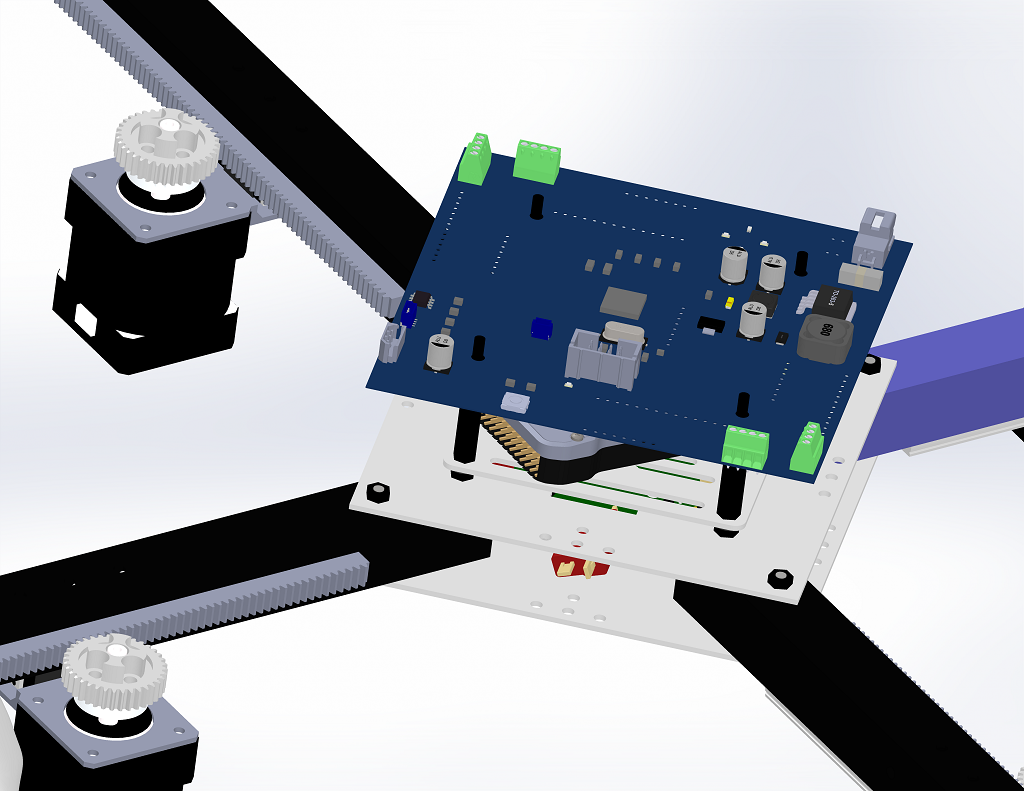
\includegraphics[width=0.9\textwidth]{figures/arducopter_slot_pcb.png}
	\caption{3D model elektroničkog sklopovlja}
	\label{Slika:3D_PCB}
\end{figure}

\subsection{Sastavni dijelovi elektroničkog slopovlja}

\subsubsection{Napajanje}
Napajanje elektroničkog sklopovlja osigurano je baterijom nazivnog napona 12 V. Na ulazu napajanja dodan je osigurač iznosa 10A. Iznos osigurača je projektiran prema maksimalnim iznosima struja koje se mogu ostvariti na koračnim motorima. Dodatno, značajniji potrošači na ovom sklopovlju su Dynamixel motori, čije je sučelje dodano za daljnja proširenja funkcionalnosti letjelice.
U sklopu modula napajanja, potrebno je osigurati stabilne iznose napona 3.3 V i 5V. Prva razina spuštanja ulaznog napona je osigurana 5V regulatorom napona, switching tipa. Specifikacije regulatora su prikazane tablicom \ref{tab:specifikacija_5V}.


\begin{table}[H]
	\centering
	\caption{Specifikacije 5V regulatora napona: }
	\label{tab:specifikacija_5V}
	\begin{tabular}{|l|c|}
		\hline
		\textbf{Proizvođač} & Texas instuments  \\ \hline 
		\textbf{Model} &  LM2592HVS-5.0  \\ \hline 
		\textbf{Tip} &  Buck(Step Down) Switching Regulator  \\ \hline 
		\textbf{Minimalni ulazni napon} & 4.5 V \\ \hline 
		\textbf{Maksimalni ulazni napon} & 60 V \\ \hline 
		\textbf{Izlazni napon} & 5 V \\ \hline 
		\textbf{Izlazna struja} & 2 A \\ \hline 
		\textbf{Frekvencija rada} & 150 kHz \\ \hline 
		\textbf{Maksimalna radna temperatura} & $125 \deg C$ \\ \hline 
	\end{tabular}
\end{table}

Nadalje, napon iznosa 3.3 V osiguran je snižavanjem 5V napona iz prethodno opisanog regulatora. U ovom slučaju korišten je linearni regulator. Korištenje ovog tipa regulatora je moguće, budući da je snaga potrošača spojenih na napajanje 3.3 V daleko manja od maksimalnog iznosa struje koju daje 5 V regulator. Specifikacije 3.3 V regulatora prikazane su tablicom \ref{tab:specifikacija_3V3}

\begin{table}[H]
	\centering
	\caption{Specifikacije 3.3V regulatora napona: }
	\label{tab:specifikacija_3V3}
	\begin{tabular}{|l|c|}
		\hline
		\textbf{Proizvođač} & ST Microelectronics \\ \hline 
		\textbf{Model} &  LD1117S33TR \\ \hline 
		\textbf{Tip} &  Fixed LDO Voltage Regulator  \\ \hline 
		\textbf{Minimalni ulazni napon} & 4.75 V \\ \hline 
		\textbf{Maksimalni ulazni napon} & 15 V \\ \hline 
		\textbf{Izlazni napon} & 3.3 V \\ \hline 
		\textbf{Izlazna struja} & 800 mA \\ \hline 
		\textbf{Maksimalna radna temperatura} & $125 \deg C$ \\ \hline 
	\end{tabular}
\end{table}

U sklopu modula napajanja, potrebno je osigurati i napajanje koračnih motora te napajanje Dynamixel motora. U ovom slučaju, koristi se ulazni napon, međutim dodani su jumperi, kako bi na jednostavan način bilo moguće odspojiti navedene potrošače u fazi programiranja elektroničkog sklopovlja.

\subsubsection{Mikrokontroler}
 Elektroničko sklopovlje je bazirano na mikrokontroleru STM32, serije F4. Jezgra mikrokontrolera je zasnovana na jezgri ARM(R) Cortex$^{TM}$-M4, 32-bit, RISC arhitekture. Na mikrokontroler su povezane sve komponente kojima je potrebno upravljati i s kojih je potrebno očitavati stanja. Specifikacije mikrokontrolera su prikazane tablicom \ref{tab:specifikacija_MCU}.

\begin{table}[H]
	\centering
	\caption{Specifikacije STM mikrokontrolera: }
	\label{tab:specifikacija_MCU}
	\begin{tabular}{|l|c|}
		\hline
		\textbf{Proizvođač} & ST Microelectronics \\ \hline 
		\textbf{Model} &  STM32F405RGT6V \\ \hline 
		\textbf{Jezgra} &  ARM(R) Cortex$^{TM}$-M4, 32-bit, RISC  \\ \hline 
		\textbf{CPU brzina} & 168 MHz \\ \hline 
		\textbf{Veličina RAM memorije} & 192 KB \\ \hline 
		\textbf{Broj pinova} & 64 \\ \hline 
		\textbf{Broj I/O jedinica} & 51 \\ \hline 
		\textbf{Ugrađena sučelja} & CAN, I2C, SPI, UART, USART, USB\\ \hline 
		\textbf{Minimalni napon napajanja} & 1.8 V\\ \hline 
		\textbf{Maksimalni napon napajanja} & 3.6 V\\ \hline 
	\end{tabular}
\end{table}

Napajanje mikrokontrolera je osigurano reguliranim naponom iznosa 3.3 V. Dodatno stabiliziranje napona je osigurano dodavanjem kondenzatora različitih iznosa. Dodatni kondenzatori su smješteni u neposrednoj blizini mikrokontrolera na tiskanoj pločici.
Za izvor takta mikrokontrolera korišten je kristalni oscilator nazivne frekvencije 8 Mhz.

\subsubsection{LED indikatori}
Prilikom izrade prototipa elektroničkog sklopovlja utvrđena je potreba postojanja LED indikatora. LED indikatori se koriste u svrhu provjere ispravnosti rada programske potpore. U ovom slučaju, dodane su 4 LED diode različitih boja. LED diode su spojene na mikorokontroler, a za izvor napajanja se koristi regulirani napon iznosa 5V. Upravljanje LED diodama je ostvareno mikrokontrolerom i bipolarnim NPN tranzistorom. Struja koja protječe LED diodom prilikom visoke razine upravljačkog signala iz mikrokontrolera je ograničena dodavanjem otpornika iznosa 500 V. 

\begin{table}[H]
	\centering
	\caption{Specifikacije LED dioda: }
	\label{tab:specifikacija_MCU}
	\begin{tabular}{|l|c|}
		\hline
		\textbf{Proizvođač} & Kingbright \\ \hline 
		\textbf{Model} & KPT-2012SECK \\ \hline 
		\textbf{Footprint} & SMD, 0805  \\ \hline 
		\textbf{Korištene boje} & crvena, naranasta, plava, žuta, zelena \\ \hline 
		\textbf{Veličina RAM memorije} & 192 KB \\ \hline 
		\textbf{Broj pinova} & 64 \\ \hline 
		\textbf{Broj I/O jedinica} & 51 \\ \hline 
		\textbf{Ugrađena sučelja} & CAN, I2C, SPI, UART, USART, USB\\ \hline 
		\textbf{Minimalni napon napajanja} & 1.8 V\\ \hline 
		\textbf{Maksimalni napon napajanja} & 3.6 V\\ \hline 
	\end{tabular}
\end{table}


\subsubsection{Pogon koračnih motora}
\subsubsection{Konektori}
\subsubsection{Dynamixel}
\subsubsection{CAN}

\subsection{Tiskana pločica - PCB}


\end{document}